\documentclass{standalone}
\usepackage{tikz}
\usepackage{ctex,siunitx}
\setCJKmainfont{Noto Serif CJK SC}
\usepackage{tkz-euclide}
\usepackage{amsmath}
\usetikzlibrary{patterns, calc}
\usetikzlibrary {decorations.pathmorphing, decorations.pathreplacing, decorations.shapes,}
\tikzset{
  tractor/.pic={
    \draw[thick](0,-0.4)rectangle(0.6,0.4);
    \draw[thick](0.6,-0.15)rectangle(1.2,0.15);
    \draw[pattern=vertical lines](0.6,0.15)rectangle(1.3,0.35);
    \draw[pattern=vertical lines](0.6,-0.15)rectangle(1.3,-0.35);
  }
}
\begin{document}
\small
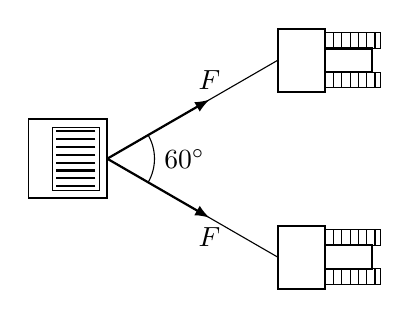
\begin{tikzpicture}[>=latex,scale=1.0]
  % \useasboundingbox(-0.25,-0.25)rectangle(4,3);
  \draw(0,0)--(30:2.5)(0,0)--(-30:2.5);
  \draw[thick,->](0,0)--(30:1.5)node[above]{$F$};
  \draw[thick,->](0,0)--(-30:1.5)node[below]{$F$};
  \draw[thin](-30:0.6)arc(-30:30:0.6)node[midway,right]{\ang{60}};
  \draw[semithick](0,-0.5)rectangle(-1,0.5);
  \draw(-0.1,-0.4)rectangle(-0.7,0.4);
  \foreach \x in {0.35,0.25,0.15,0.05,-0.05,-0.15,-0.25,-0.35}
  { \draw[thick](-0.15,\x)--++(-0.5,0);}
  \pic at (30:2.5){tractor};
  \pic at (-30:2.5){tractor};
\end{tikzpicture}
\end{document}